
\gr
\chapter{Εκτίμηση μεταβλητότητας καρδιακού ρυθμού}
\section{Μετρικές εκτίμησης μεταβλητότητας καρδιακού ρυθμού}
Στο προηγούμενο κεφάλαιο παρουσιάστηκε ο ορισμός της καρδιακής μεταβλητότητας (\en Heart Rate Variability, HRV \gr) και η βαρύτητα που διαθέτει ως προς την αξιολόγηση της φυσιολογικής λειτουργίας της καρδιάς. Η αξιολόγηση και η μέτρηση αυτή πραγματοποιείται με χρήση διαφορετικών μετρικών. Οι δύο βασικές κατηγορίες μετρικών είναι οι γραμμικές και οι μη γραμμικές και στη συνέχεια οι γραμμικές μέθοδοι χωρίζονται σε δύο επιπλέον κατηγορίες, τις μετρικές στο χώρο του χρόνου και τις μετρικές στο χώρο της συχνότητας. Σε αυτό το κεφάλαιο θα αναλυθούν οι συγκεκριμένες μετρικές και η σημαντικότητά τους ως προς την αξιολόγηση του \en HRV. \gr
\subsection{Γραμμικές μέθοδοι}
\textbf{\\ Μέθοδοι στο πεδίο του χρόνου}
\par
Οι μετρικές στο πεδίο του χρόνου αντικατοπτρίζουν τη μεταβλητότητα ανάμεσα στους διαδοχικούς καρδιακούς παλμούς. Συνήθως εκφράζονται σε αρχικές μονάδες ή σε μορφή λογαρίθμου (πιο συγκεκριμένα του φυσικού λογαρίθμου \en ln() \gr για μια πιο κανονική κατανομή). 
\par
Το πλεονέκτημά του σε σύγκριση με αυτό της συχνότητας, είναι ότι οι μετρήσεις που παράγουν τους ανάλογους δείκτες γίνονται απευθείας επάνω στο σήμα και υπάρχει μόνο ένας τρόπος υπολογι\-σμού. Οι διάφοροι αυτοί δείκτες υπολογίζονται με βάση τα ονομαζόμενα ΝΝ-διαστήματα \en (NN intervals, N = normal), \gr  συνώνυμα των \en RR \gr διαστημάτων, με τη διαφορά ότι επιλέγονται μόνο Ν χτύποι, δηλαδή χτύποι που 
προέρχονται από εκπολώσεις του φλεβόκομβου. Οι δείκτες που προκύπτουν χωρίζονται σε δύο κατηγορίες, τη στατιστική και τη γεωμετρική.

\par
Στον παρακάτω πίνακα παρουσιάζονται σχεδιαγραμματικά οι μετρικές στο πεδίο του χρόνου και έπειτα η ανάλυση της κάθε μίας ξεχωριστά (Πίνακας 3.1).

\begin{center}
	\begin{longtable}{l l l}
		\caption{Μετρικές στο πεδίο του χρόνου} \\
		\centering 
		Όνομα παραμέτρου & Μονάδες μέτρησης & Περιγραφή \\ [0.5ex] 
		\endfirsthead
		\hline \hline \en 
		\en SDNN & \en $ms$ & Τυπική απόκλιση ΝΝ διαστημάτων \\ [1ex] 
		\en SDRR & \en $ms$ & Τυπική απόκλιση \en RR \gr διαστημάτων  \\ [1ex] 
		\en SDANN & \en $ms$ & Τυπική απόκλιση των μέσων \\ 
		& & διαστημάτων NN για \\
		& & κάθε τμήμα 5 λεπτών σε μια\\
		& & 24 ωρη καταγραφή \\ [1ex] 
		\en SDNN \\
		\en index \\
		\en (SDNNI) & \en $ms$ & Μέσος όρος των \\
		& & τυπικών αποκλίσεων όλων των \\ 
		& & διαστημάτων NN για κάθε τμήμα 5  \\
		& & λεπτών μιας 24 ωρης εγγραφής \\ [1ex] 
		\en pNN50 & $\%$ & Ποσοστό διαδοχικών διαστημάτων  \\
		& & \en RR \gr με χρονική διαφορά\\
		& & μεγαλύτερη των 50 \en ms\\ [1ex] 
		\en HR Max \& \\
		\en HR Min &\en $bpm$ & Μέση διαφορά μεταξύ των υψηλότερων \\
		& & και των χαμηλότερων καρδιακών \\
		& & παλμών κατά τη διάρκεια κάθε\\
		& & αναπνευστικού κύκλου \\ [1ex] 
		\en RMSSD & \en $ms$ & Τετραγωνική ρίζα διαδοχικών\\
		& & διαφορών διαστήματος \en RR\\ [1ex] 
		\en HRV \\
		\en triangular \\
		\en index & - & Ολοκλήρωμα της πυκνότητας \\
		& & του ιστογράμματος διαστήματος \en RR \gr \\
		& & διαιρεμένο με το ύψος του \\ [1ex] 
		\en TINN & \en $ms$ & Πλάτος βάσης του ιστογράμματος \\
		& & διαστήματος \en RR \gr \\ [1ex] 
		\hline 
	\end{longtable}
\end{center}

\begin{itemize}
	\item Στατιστικές μέθοδοι: Προκύπτουν από καταγραφές σημάτων μεγάλης διάρκειας που φτάνουν τις 24 ώρες. Οι τιμές τους αποκτώνται είτε από απευθείας μετρήσεις των ΝΝ διαστημάτων είτε μετά από επεξεργασία (αριθμητικές διαφορές ανάμεσα στις τιμές των διαστημάτων ΝΝ). Μερικοί από τους δείκτες που προκύπτουν χωρίς τη χρήση των διαφορών των διαστημάτων είναι οι
	\begin{itemize}
		\item \en SDNN
		\item SDANN \gr
	\end{itemize}
	Από τους πιο κοινούς δείκτες που προκύπτουν από διαφορά ανάμεσα σε ΝΝ διαστήματα είναι οι
	\begin{itemize}
		\item \en RMSSD
		\item SDNNi
		\item SDSD
		\item NN50 count
		\item pNN50 \gr
	\end{itemize}
	\item Γεωμετρικές μέθοδοι: Οι γεωμετρικές μέθοδοι χαρακτηρίζονται από μεγαλύτερη ανθεκτικότητα όσον αφορά στην ποιότητα των δεδομένων που συλλέγονται. Η διαφορά τους με τις στατιστικές μεθόδους είναι η διάρκεια των διαστημάτων των μετρήσεων, που φτάνουν έως και τα είκοσι λεπτά. Οι ακολουθίες των ΝΝ διαστημάτων μπορούν να μελετηθούν μέσω της μετατροπής τους σε γεωμετρικά μοτίβα. Τα μοτίβα που παράγονται μπορούν να προσεγγιστούν με δύο διαφορετικούς τρόπους. Ο πρώτος τρόπος είναι οι βασικές μετρήσεις των γεωμετρικών μοτίβων, παραδείγματος χάριν, εκτίμηση της μέγιστης τιμής του άξονα Χ ή \en Y \gr (π.χ. η τιμή του \en HRV triangular index \gr, δίνεται, μέσω του διαγράμματος της εικόνας, ως ο λόγος \en D/Y \gr). O δεύτερος τρόπος είναι η παρεμβολή μαθηματικού σχήματος στο γεωμετρικό μοτίβο, δηλαδή η προσέγγιση της κατανομής του ιστογράμματος με ένα τρίγωνο. Η αναγωγή αυτή, στη συνέχεια, χρησιμοποιείται για την εκτίμηση του ΤΙΝΝ (ΤΙΝΝ = Β-Α).
	Οι γεωμετρικές μέθοδοι χρησιμοποιούν την ακολουθία των ΝΝ διαστημάτων για τη μετατροπή, η οποία οδηγεί στη δημιουργία ιστογραμμάτων. Οι τέσσερις πιο συνηθισμένοι δείκτες μέτρησης των γεωμετρικών μεθόδων είναι οι: 
	\begin{itemize}
		\item \en HRV triangular index \gr: Προκύπτει από τη χρήση εικοσιτετράωρων μετρήσεων και ορίζεται ως το ολοκλήρωμα της πυκνότητας του ιστογράμματος των \en RR \gr διαστημάτων διαιρεμένο με το ύψος του ιστογράμματος.
		\item ΤΙΝΝ: Το πλάτος του ιστογράμματος των \en RR \gr διαστημάτων (μονάδα μέτρησης: \en $ms$).\gr
		\item \en Differential index: \gr Διαφορές του πλάτους του ιστογράμματος διαφορών ανάμεσα σε γειτονικά ΝΝ διαστήματα μετρημένα σε συγκεκριμένα ύψη (μονάδα μέτρησης: \en $ms$).\gr
		\item \en Logarithmic index \gr: Συντελεστής φ της αρνητικά εκθετικής καμπύλης \en k * e - \gr φ \en t.
	\end{itemize}
\end{itemize}
\gr
\textbf{\\ Μέθοδοι στο πεδίο της συχνότητας}
\par
Οι μέθοδοι στο πεδίο της συχνότητας εκτιμούν την κατανομή (απόλυτης και σχετικής) ισχύος σε τέσσερις βασικές ζώνες συχνότητας και οι καταγραφές κυμαίνονται σε διάρκεια είτε από 2-5 λεπτά είτε 24 ώρες. Οι ζώνες αυτές είναι ονομαστικά οι: υπέρ χαμηλές συχνότητες, πολύ χαμηλές συχνότητες, χαμηλές συχνότητες και υψηλές συχνότητες. Η κατηγοριοποίηση των μετρικών και παρουσιάζονται στον ακόλουθο πίνακα (Πίνακας 3.2):

\begin{center}
	\begin{longtable}{l l l}
		\caption{Μετρικές στο πεδίο της συχνότητας}\\
		\centering 
		Όνομα παραμέτρου & Μονάδες μέτρησης & Περιγραφή \\ [0.5ex] 
		\hline \hline \en 
		\en ULF power & \en $ms^2$ & \gr Απόλυτη ισχύς της ζώνης εξαιρετικά \\ 
		& & χαμηλών συχνοτήτων ($\leq 0,003 Hz$)\\ [1ex] 
		\en VLF power & \en $ms$ & Απόλυτη ισχύς της ζώνης πολύ \\
		& & χαμηλής συχνότητας ($0,0033 - 0,04 Hz$)  \\ [1ex] 
		\en  LF peak & \en $Hz$ & Συχνότητα κορυφής της ζώνης χαμηλής\\
		& & συχνότητας ($0,04 - 0,15 Hz$)\\ [1ex] 
		\en LF power index & \en $ms^2$ & Απόλυτη ισχύς της ζώνης χαμηλής \\
		& & συχνότητας ($0,04 - 0,15 Hz$)\\ [1ex] 
		\en LF power & $nu$ & Σχετική ισχύς της ζώνης χαμηλής \\
		& & συχνότητας ($0,04 - 0,15 Hz$) σε \\
		& & κανονικές μονάδες \\ [1ex] 
		\en LF power & \en \% & Σχετική ισχύς της ζώνης χαμηλής \\
		& & συχνότητας ($0,04 - 0,15 Hz$)\\ [1ex] 
		\en HF peak & $Hz$ & Συχνότητα κορυφής της ζώνης υψηλής\\
		& & συχνότητας ($0,15 - 0,4 Hz$)\\ [1ex] 
		\en HF power & \en $nu$ & Σχετική ισχύς της ζώνης υψηλής\\
		& & συχνότητας ($0,15 - 0,4 Hz$) σε \\
		& & κανονικές μονάδες\\ [1ex] 
		\en HF power & \en \% & Σχετική ισχύς της ζώνης υψηλών\\
		& & συχνοτήτων ($0,15 - 0,4 Hz$)\\ [1ex] 
		\en LF/HF & \en \% & Λόγος \en LF/HF\\ [1ex] 
		\hline 
	\end{longtable}
\end{center}
Η κατηγοριοποίηση των μετρικών σχετικά με τη διάρκεια είναι η ακόλουθη:
\begin{itemize}
	\item Ανάλυση σύντομων καταγραφών των 5 λεπτών: συνολική ισχύς των 5 λεπτών, \en LF, LF norm [LF x 100 /(\gr Συνολική ισχύς - \en VLF)\gr (μονάδα μέτρησης: \en normalized units)], HF, HF norm [HF x 100], LF/HF. \gr
	\item Ανάλυση καταγραφών 24 ωρών: Συνολική ισχύς (Η διακύμανση όλων των ΝΝ διαστημάτων), \en ULF, LF, HF, \gr α (Κλίση της γραμμικής παρεμβολής του φάσματος στην \en log-log \gr  κλίμακα) [11]-[17], [45].
\end{itemize}
\par
\textbf{\\ Kυματίδια \en Haar \gr}
\par
Στον κλάδο των μαθηματικών, το κυματίδιο \en Haar \gr είναι μία ακολουθία εναλλασσόμενων συναρτήσεων με μορφή "τετράγωνων κυματομορφών". Αυτές οι συναρτήσεις αποτελούν μία ολόκληρη οικογένεια κυματιδίων και χρησιμοποιούνται σε ποικίλους κλάδους για την εξαγωγή πληροφοριών από σήματα. Η ανάλυση με χρήση κυματιδίων μοιάζει με την ανάλυση \en Fourier, \gr διότι επιτρέπει  σε μία συνάρτηση να αναπαρασταθει μέσω μιας ορθοκανονικής βάσης. 
\par
Προτάθηκε το 1909 από τον Ούγγρο μαθηματικό \en Alfred Haar, \gr  ο οποίος χρησιμοποίησε αυτές τις συναρτήσεις για να ορίσει ένα ορθοκανονικό σύστημα στο χώρο των τετραγωνικών συναρτήσεων (για το μοναδιαίο διάστημα [0, 1]). Τα κυματίδια \en Haar \gr αποτελούν ειδική περίπτωση των κυματιδίων \en Daubechies \gr (μια οικογένεια ορθογώνιων κυματιδίων) που είναι επίσης γνωστά ως \en Db1 \gr.
\par
\begin{figure}[!ht]
	\centering
	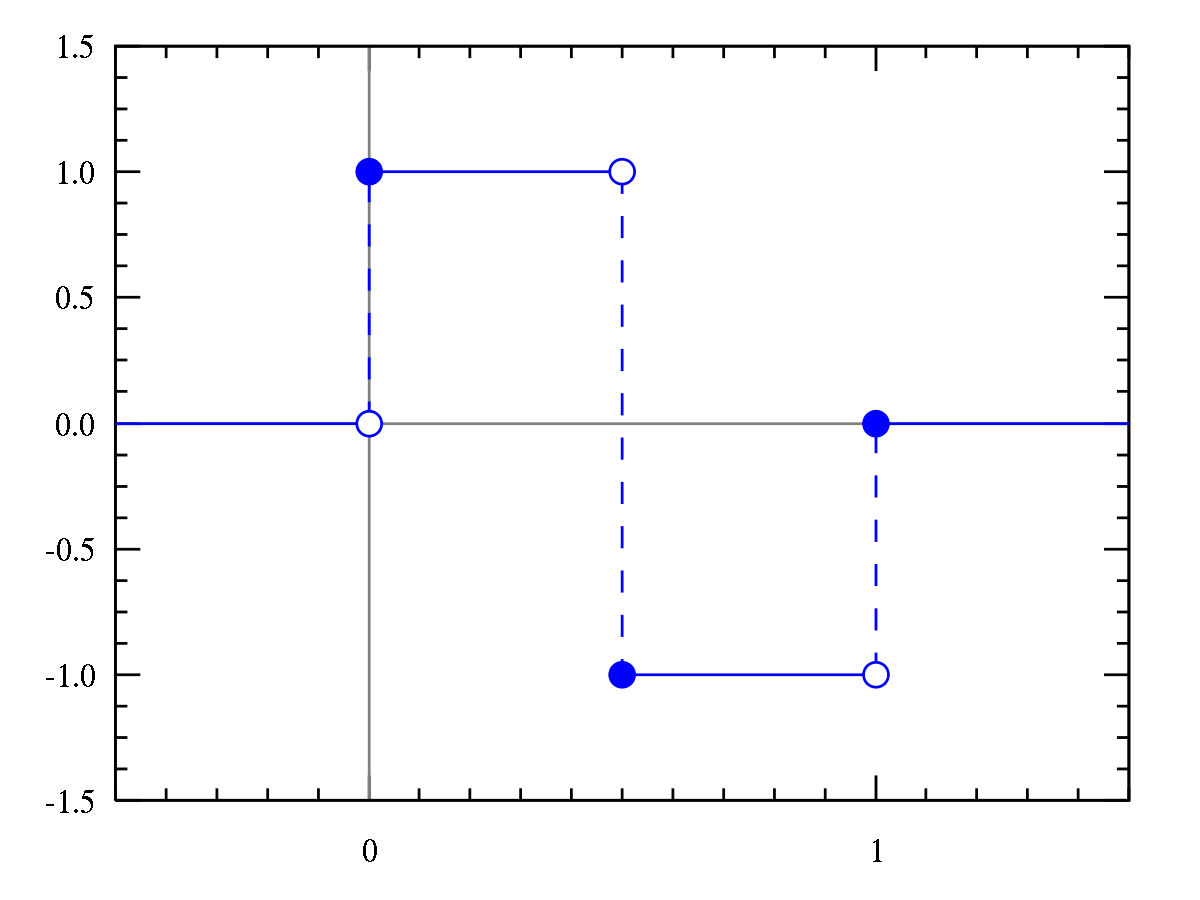
\includegraphics[scale = 0.2]{haar.png}    
	\caption{\gr Κυματίδια \en Haar \protect\url{en.wikipedia.org} \gr}
\end{figure}
Τα κυματίδια \en Haar \gr αποτελούν την πιο απλή μορφή κυματιδίων. Έχουν το εξής ελάττωμα: δεν είναι συνεχή και επομένως δεν είναι παραγωγίσημα. Για τα διακριτά σήματα, όμως, αυτό μπορεί να αποτελέσει πλεονέκτημα. Από την άλλη, ένα πλεονέκτημά τους είναι η ολοκλήρωσή τους λόγω της γραμμικότητάς τους. Ένα ακόμα χαρακτηριστικό τους είναι το εύρος των τιμών που λαμβάνουν, το οποίο αντιστοιχεί σε μόλις 3 αριθμούς: 0, 1, -1. 
\par
Οι τιμές που λαμβάνουν οι συναρτήσεις των κυματιδίων δίνονται από την παρακάτω ακολουθία για το διάστημα 0, 1:
\begin{equation}
	h_i (x) = \begin{cases}
		\text{ 1,  για } x \in [\xi 1, \xi2), \\
		\text{-1, για } x \in [\xi 2, \xi 3), \\
		\text{ 0, αλλιώς}
	\end{cases}
\end{equation}
όπου $\xi 1 = \frac{k}{m}, \xi 2 = \frac{k + 0.5}{m}, \xi 3 = \frac{k + 1}{m}$.
\par\par
Η παράμετρος $m = 2^j, j = 0, 1, ..., J$ δηλώνει το επίπεδο του κυματίου και το $k = 0, 1, ..., m-1$ την παράμετρο μετάφρασης. Ο δείκτης $i$ δίνεται από τη σχέση $i = m + k - 1$. Οι ελάχιστές τιμές είναι  $m = 1, k = 0 $ που δίνουν $i = 2$ και η μέγιστη τιμή του δείκτη είναι $i = 2M = 2J + 1$. [46]-[53]
\par
Αποτελέσματα της χρήσης των κυματιδίων \en Haar \gr στην επεξεργασία σημάτων φαίνεται στην ακόλoυθη εικόνα. Στα αριστερά φαίνεται μια διακριτή χρονοσειρά και στα αριστερά η προσέγγισή της με κυματίδια \en Haar \gr:
\begin{figure}[h!]
	\centering
	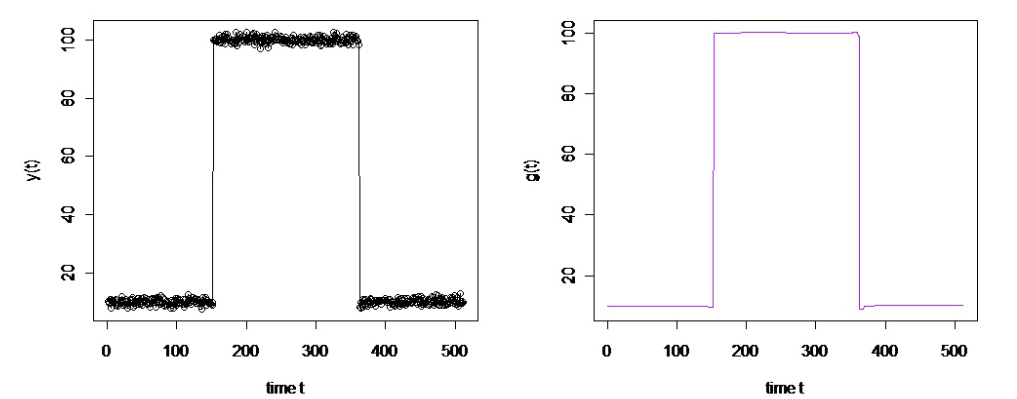
\includegraphics[scale = 0.4]{haar2.png}    
	\caption{\gr Εφαρμογή κυματιδίων \en Haar \gr για συλλογή πληροφοριών από σήμα \en\protect\url{commons.wikimedia.org}}
\end{figure}
\subsection{Μη γραμμικές μέθοδοι}
Σε αυτή την κατηγορία η σχέση των μεταβλητών δεν απεικονίζεται γραμμικά, δηλαδή σε μια ευθεία γραμμή. Οι μη γραμμικές μέθοδοι συνδέονται με την πολυπλοκότητα και την προβλεψιμότητα του σήματος (χρονοσειρά). Οι μη γραμμικές μέθοδοι μας επιτρέπουν να υπολογίσουμε ποσοτικά τη μη προβλεψιμότητα των χρονοσειρών, που πηγάζει από την πολυπλοκότητα των μηχανισμών που ρυθμίζουν το  \en HRV \gr. Για την παρουσίαση των δεδομένων των μη γραμμικών μεθόδων χρησιμοποιείται κυρίως η αναπαράσταση του \en Poincare, \gr η οποία απεικονίζει τη συσχέτιση ανάμεσα σε διαδοχικά \en RR \gr διαστήματα. Οι μέθοδοι αυτές απεικονίζονται με τη βοήθεια της αναπαράστασης του \en Poincare \gr, η οποία αποτελεί ένα χάρτη σημείων στο σύστημα των καρτεσιανών συντεταγμένων φτιαγμένο από τις τιμές των \en RR \gr
διαστημάτων. Αυτή η αναπαράσταση βοηθά στο να εξηγηθούν οι παρακάτω μετρήσεις:\begin{itemize}
	\item \en S: \gr Το εμβαδό της έλλειψης που αντιστοιχεί στο ολικό \en HRV. \gr
	\item \en SD1: \gr Η τυπική απόκλιση (εξ ου και το \en SD \gr) της απόστασης κάθε σημείου από τον άξονα $y=x$, καταδεικνύει το πλάτος της έλλειψης.
	\item \en SD2: \gr Η τυπική απόκλιση της απόστασης κάθε σημείου από τον άξονα $y=x +$ το μέσο \en RR \gr διάστημα, καταδεικνύει το μήκος της έλλειψης. 
	\item \en SD1/SD2: \gr Μετρά τη μη προβλεψιμότητα των \en RR \gr διαστημάτων και συσχετίζεται με το λόγο \en LF/HF. \gr
	\item \en ApEn: Approximate Entropy\gr , μετρά την κανονικότητα και την πολυπλοκότητα μιας χρονοσειράς. Υψηλές τιμές δείχμουν χαμηλή προβλειμότητα της διακύμανσης σε διαδοχικά \en RR \gr διαστήματα.
	\item \en SampEn: Sample Entropy \gr, μετρά την κανονικότητα και την πολυπλοκότητα μιας χρονοσειράς. Σχεδιάστηκε για πιο έμπιστες μετρήσεις και μπορεί να υπολογιστεί σε μικρότερες χρονοσειρές από την \en ApEn \gr.
	\item \en DFA \gr α1: \en Detrended Fluctuation Analysis,\gr υπολογίζει συσχέτιση διαδοχικών RR διαστημάτων. Η κλίση α1 περιγράφει σύντομες εναλλαγές.
	\item \en DFA \gr α2: Η κλίση α2 περιγράφει εναλλαγές μεγαλύτερης διάρκειας από την α1. 
	\item \en D2: \gr Εκτιμά τον ελάχιστο αριθμό μεταβλητών που χρειάζονται για να κατασκευαστεί ένα μοντέλο δυναμικού συστήματος \en (system dynamics, \gr μοντελοποίηση που βοηθά στην κατανόηση μη γραμμικής συμπεριφοράς).
\end{itemize}[44].
\section{Μέθοδοι εκτίμησης μεταβλητότητας καρδιακού ρυθμού}
\subsection{Εντροπία και μέθοδοι εκτίμησης}
Η έννοια της εντροπίας βρίσκει εφαρμογή σε ποικίλους επιστημονικούς κλάδους, κάποιες φορές με πιο αυστηρούς μαθηματικούς ορισμούς και άλλοτε πιο αφηρημένα. Χρησιμοποιείται ευρέως στη φυσική, την κβανοτμηχανική και τη θεωρία πληροφορίας με την επεξεργασία χρονοσειρών. Χρησιμοποιήθηκε και ορίστηκε πρώτη φορά στην εισαγωγή των θερμοδυναμικών συστημάτων (μακροσκοπικός κόσμος) με τον \en Clausius, \gr όταν έθεσε τις πρώτες βασικές έννοιες της εντροπίας στο πλαίσιο της θερμοδυναμικής. Η επιλογή της λέξης «εντροπία» ήταν σκόπιμη, για να τονιστεί η άμεση σύνδεση της εντροπίας με την ενέργεια. Πιο στοχευμένα, όμως, στην παρούσα διπλωματική εργασία οι μέθοδοι εκτίμησης της εντροπίας αντιστοιχούν στους παρακάτω ορισμούς: 
\begin{itemize}
	\item \en Shannon: \gr Στη θεωρία πληροφορίας, ο \en Shannon \gr  όρισε την εντροπία ως έναν τρόπο μέτρησης της αβεβαιότητας της πληροφορίας μιας γραμματοσειράς, χρησιμοποιώντας την στο σύστημα επικοινωνίας. Το σύστημα αυτό αποτελείται από έναν πομπό, ένα δίαυλο μέσω του οποίου εκπέμπεται ένα κωδικοποιημένο σήμα και έναν παραλήπτη, ο οποίος αποκωδικοποιεί το σήμα. Ο \en Shannon \gr όρισε δύο κύριες έννοιές της θεωρίας πληροφορίας: την ποσότητα πληροφορίας και την ομώνυμη εντροπία πληροφορίας. Η ποσότητα πληροφορίας ορίζεται ως:
	\begin{equation}
		I = K ln (M)
	\end{equation}
	με Ι τη συνολική πληροφορία του μηνύματος (συμβολοσειρά), Κ μια σταθερά που επιτρέπει την αλλαγή βάσης του λογαρίθμου, που ισοδυναμεί με την αλλαγή της μονάδας αναπαράστασης της πληροφορίας (π.χ. \en bits \gr). Αν επιλεχθεί το σωστό Κ είναι δυνατή η χρήση οποιασδήποτε λογαριθμικής βάσης. Τέλος, Μ είναι ο συνολικός αριθμός των πιθανών μηνυμάτων ενός πεπερασμένου συνόλου. [59]
	\item \en Rényi: \gr Αυτή η εντροπία αποτελεί γενίκευση της προηγούμενης και όπως η εντροπία του \en Shannon, \gr χρησιμοποιείται και αυτή για τη μέτρηση αβεβαιότητας ενός σήματος. Σε αυτή την περίπτωση υπάρχει η προσθήκη μιας παραμέτρου $\alpha$ (τάξη) που απεικονίζει συχνά ή και σπάνια φαινόμενα. Τα διαφορετικά φαινόμενα αντιστοιχούν σε διαφορετικές τιμές της παραμέτρου και του τύπου εντροπίας. Ο γενικός τύπος του \en Renyi \gr τάξης $\alpha$, \gr με $\alpha \geq 0$ και $\alpha \neq 1$
	\begin{equation}
		H_\alpha (X) = \frac{1}{1 - \alpha} log_2 (\sum_{i=1}^{n}{p_i^\alpha})
	\end{equation}
	όπου η μεταβλητή Χ είναι διακριτή και τυχαία. Η ποσότητα \en $H_\alpha (X)$ \gr είναι μέτρο της εντροπίας της κατανομής $ X = (x_1, ..., x_n)$, μονότονη και μη φθίνουσα συνάρτηση του $\alpha$. Οι ποσότητες $p_i$ είναι οι αντίστοιχες πιθανότητες εμφάνισης.
	\par
	Οι πιο συνηθισμένες τιμές της παραμέτρου είναι οι:
	\begin{itemize}
		\item $\alpha = 1$: Όταν το $\alpha$ συγκλίνει προς το 1, τότε λαμβάνουμε την εντροπία του \en Shannon: \gr
		\begin{equation}
			H_1 (X) = \lim_{\alpha \to 1}
		\end{equation}
		\begin{equation}
			H_\alpha (X) = - \sum_{i=1}^{n}{p_i} log (p_i)
		\end{equation}
		
		\item $\alpha = 2$: Εντροπία του \en Rényi. \gr Όταν η τιμή της τάξης δεν προσδιορίζεται, ως βάση θεωρείται ο αριθμός 2. Αυτή η περίπτωση ονομάζεται επίσης εντροπία σύγκρουσης, και οι μεταβλητές Χ, Υ θεωρούνται ανεξάρτητες.
		\begin{equation}
			H_2 (X) = - log\sum_{i=1}^{n}{p_i^2} = log P(X = Y)
		\end{equation}
		
		\item $\alpha = 0$: Μέγιστη εντροπία. Υποθέτεται πως όλες οι πιθανότητες είναι θετικές και τότε ως εντροπία ορίζεται ο λογάριθμος του πλήθους των τιμών που μπορεί να λάβει το Χ.
		\begin{equation}
			H_0 (X) = log n = log |X|
		\end{equation}
		
		\item $\alpha = \infty$: Ελάχιστη εντροπία και ελάχιστη τιμή της εντροπίας του \en Rényi. \gr και το αποτέλεσμα συγκλίνει στον αρνητικό λογάριθμο της μέγιστης πιθανότητας.
	\end{itemize}
	
	Οι μέχρι στιγμής ορισμοί και μέθοδοι εντροπίας αφορούν μόνο στο φυσικό κόσμο και τις διαστάσεις του. Η ευρέως χρησιμοποιούμενη εντροπία του \en  Shannon \gr δεν εμβαθύνει σε χώρους μεγαλύτερης διάστασης, κάτι πολύ χρήσιμο σε διαφορετικούς κλάδους, όπως η Ιατρική Πληροφορική. Η μελέτη  του καρδιακού παλμού και του \en HRV \gr κάνει αναγκαία την εύρεση μεθόδων που εμβαθύνουν στον \en m\gr-διάστατο χώρο. Στη συνέχεια παραθέτονται και αναλύονται κάποιες από αυτές τις βασικές μεθόδους εκτίμησης της εντροπίας σε αυτόν. [54]-[58]
\end{itemize}
\subsection{Εκτίμηση εντροπίας στο \en m-\gr διάστατο χώρο}
Για λόγους πρακτικότητας θα αποφευχθεί η αναλυτική παρουσίαση των μεθόδων που δε χρησιμοποιήθηκαν σε αυτή τη διπλωματική. Θα παρουσιαστούν, θα εξηγηθούν αλλά δε θα αναλυθούν στον ίδιο βαθμό με αυτές που χρησιμοποιήθηκαν. Ο λόγος που δε χρησιμοποιήθηκαν όλες οι παρακάτω μέθοδοι είναι ότι δεν είναι όλες εφαρμόσιμες στο χώρο ανάλυσης καρδιακών σημάτων. 
\subsubsection{ \en Permutation Entropy \gr ή Εντροπία αντιμετάθεσης}
Aποτελεί μέτρο εκτίμησης πολυπλοκότητας μιας χρονοσειράς. Είναι ένας απλός, υπολογιστικά φθηνός αλγόριθμος που μπορεί να εφαρμοστεί σε σήματα μικρού μήκους. Επιπλέον, λαμβάνει υπόψη τη χρονική σειρά των τιμών στο σήμα, σε αντίθεση με την εντροπία του \en Shannon, \gr επομένως στην \en Permutation Entropy \gr οι δύο χρονοσειρές $X_1 = \{1, 0, 1, 0\}$ και $X_2 = \{1, 0, 0, 1\}$ δε θα δίνουν το ίδιο αποτέλεσμα [60]. 
\par
\begin{figure}[!ht]
	\centering
	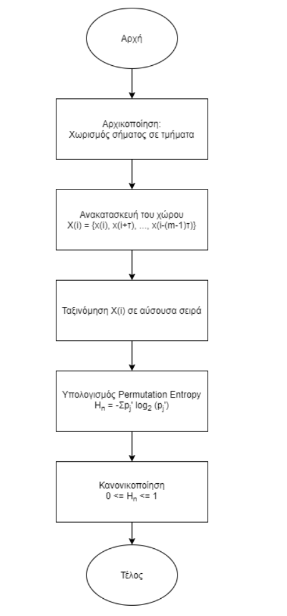
\includegraphics{Permutation.png}    \caption{Βήματα αλγορίθμου της \en Permutation Entropy\gr }
\end{figure}
\par
Τα βήματα του αλγορίθμου παρουσιάζονται επιγραμματικά στο ακόλουθο σχεδιάγραμμα (Σχήμα 3.3). 

\subsubsection{ \en Approximate Entropy (ApEn) \gr}
Ορίστηκε πρώτη φορά το 1995, από τον \en Steve Pincus,\gr  αποτελεί αλγόριθμο εκτίμησης της πολυπλοκότητας μιας χρονοσειράς και. Βασιζόμενη στη Θεωρία Πληροφορίας, εφαρμόζεται σε πολλούς τομείς, μερικοί από τους οποίους είναι η ιατρική, η φυσιολογία, οι τηλεπικονωνίες αλλά και η οικονομία. Η πηγή η οποία παράγει τα δεδομένα δεν επηρεάζει την εφαρμογή της μεθόδου (εφαρμόζεται ανεξάρτητα από αυτή), κάτι που συμβάλλει στην επιτυχία της. Διαθέτει ανθεκτικότητα σε στοχαστικές συμπεριφορές, όπως παρουσία θορύβου. \en H ApEn \gr μελετά την πιθανότητα όμοια μοτίβα σε μια χρονοσειρά να προηγούνται άλλων πρόσθετων όμοιων δεδομένων. Η πιθανότητα επανάληψης είναι αντιστρόφως ανάλογη των τιμών που λαμβάνει, (δηλαδή μικρότερες τιμές αντιστοιχούν σε υψηλή πιθανότητα επανάληψης και αντίστροφα)ς. Οι τρεις βασικές παράμετροι του αλγόριθμου είναι το Ν (το συνολικό μέγεθος των δεδομένων), το \en m \gr (η διάσταση ενσωμάτωσης) και το \en r, \gr η παράμετρος κλίμακας (φίλτρο θορύβου). 
\par
Τα βήματα του αλγορίθμου είναι τα ακόλουθα:
\par
Βήμα 1ο: Έστω η σειρά δεδομένων $u(1), u(2), ..., u(N)$.
\par
Βήμα 2ο: Δίνονται μη αρνητικές τιμές στις παραμέτρους, με $m \leq N$. 
\par
Βήμα 3ο: Ορισμός μιας ακολουθίας διανυσμάτων $x(1), x(2), ..., x(N-m+1)$ στο \en m-\gr διάστατο χώρο $\Re^m$. Τα διανύσματα ορίζονται ως: $x(i) = [u(i), u(i+1), ..., u(i+m-1)]$. Σε αντίθεση με τις προηγούμενες μεθόδους, σε αυτή τη μέθοδο γίνεται χρήση των τιμών του διανύσματος αντί των πιθανοτήτων τους. 
\par
Βήμα 4ο: Για κάθε $i$ στο διάστημα $[1, N-m+1]$, κατασκευάζεται η ακόλουθη ποσότητα με χρήση των διανυσμάτων.
\begin{equation}
	C_i^m (r) = \frac{ \gr \text{πλήθος } x(j) \text{τέτοια ώστε } \en d[x(i), x(j)] \leq r}{N-m+1}
\end{equation}
Όπου $d[x, x*] = max_a |u(a) - u*(a)|$, με $u(a)$ τα βαθμωτά μεγέθη του $x$ και $d$ η μέγιστη απόσταση μεταξύ τους. Τονίζεται πως το $j$ παίρνει όλες τις τιμές, για να συμπεριληφθεί και η ισότητα $j = i$ 
\par 
Βήμα 5ο: Ορίζεται το μέγεθος 
\begin{equation}
	\Phi^m (r) = (N-m+1)^-1 \sum_{i=1}^{N-m+1} log(C_i ^m (r))
\end{equation}
\par
Βήμα 6ο: Ορισμός της \en ApEn \gr ως:
\begin{equation}
	ApEn = \Phi^m (r) - \Phi^m+1 (r)
\end{equation}
με $log$ το φυσικό λογάριθμο για τις τιμές των $m, r$ από το 2ο βήμα.
\par 
Χαμηλές τιμές στον αλγόριθμο υποδεικνύουν ότι το υπό μελέτη σύστημα παρουσιάζει σταθερότητα, μεγάλο βαθμό επανάληψης και δεν περιέχει απρόβλεπτα μοτίβα. Το αντίθετο (υψηλές τιμές) δείχνει ανεξαρτησία ανάμεσα στα δεδομένα και μεγάλο βαθμό τυχαιότητας. Η μέγιστη τιμή που μπορεί να λάβει η \en ApEn \gr σε ένα δυαδικό σύστημα είναι $log2$ (απολύτως τυχαία δεδομένα) και τιμές μικρότερες από αυτή προβλέπουν την ύπαρξη επαναλαμβανόμενων μοντέλων. Όπως προαναφέρθηκε, είναι ανθεκτική σε διάφορες μορφές θορύβου, καθώς τιμές που αποκλίνουν πολύ σε σχέση με τις υπόλοιπες συμβάλλουν σε μικρότερο βαθμό στο συνολικό αποτέλεσμα. Λόγω της κατασκευής του αλγορίθμου και των ριζών του στη Θεωρία Πληροφορίας, η τιμή της είναι μη αρνητική και λαμβάνει την τιμή 0 για τέλειες κανονικές σειρές δεδομένων.
\par
Στον αρχικό ορισμό της \en ApEn \gr η διατήρηση της τάξης δεν είναι απόλυτη, διότι με διαφορετικούς  συνδυασμούς των παραμέτρων $ m, r$ τα αποτελέσματά της διακυμαίνονται σημαντικά. Το βασικό χαρακτηριστικό της χρησιμότητάς της είναι ότι ο βαθμός επαναληψιμότητας, δηλαδή η τυχαιότητα των δεδομένων, αρκεί για το διαχωρισμό των διάφορων συστημάτων. Τα αποτελέσματα, παρόλα αυτά, δεν είναι απόλυτα,καθώς υπάρχουν ζέυγη τιμών που δε διατηρούν αυτή την ιδιότητα. Ο \en Pincus \gr πρότεινε κάποιες προτιμώμενες τιμές σχετικά με τις παραμέτρους $m, r$. Το $m$ προτείνεται να λαμβάνει τις τιμές 2, 3 ενώ το $r$ ανήκει στο διάστημα $[0.1,0.25] std(x)$, με $std(x)$ η τυπική απόκλιση του σήματος. Δεν εφαρμόζονται, όμως, παντού μιας και διαφορετικοί τύποι δεδομένων αντιμετωπίζονται με διαφορετικό τρόπο. Βασικό ερώτημα είναι η τιμή του $r$ που πρέπει να χρησιμοποιείται σε συγκρίσεις μεταξύ διαφορετικών χρονοσειρών.
\par
Αν ισχύει $ApEn(m1, r1)(A)$ τότε ισχύει και $ApEn(m2, r2)(B)$, για κάθε ζεύγος $r2 \geq r1$. Οι προτεινόμενες τιμές ισχύουν για δεδομένα σχετικά με καρδιακό παλμό και έκκριση ορμονών αλλά όχι για δεδομένα νευρικών ώσεων. Οι μεγαλύτερη εφικτή διαφορά στη σύγκριση αποτελεσμάτων ανάμεσα στις τιμές $m, m+1$ δίνεται όταν βρεθεί η τιμή $r$ που μεγιστοποιεί την \en ApEn \gr. Η τιμή $rmax$ είναι αντιστρόφως ανάλογη του μεγέθους των δεδομένων, δηλαδή όσο η τιμή αυξάνεται τόσο μικρότερο είναι το μέγεθος των δεδομένων. Υπό αυτές τις προϋποθέσεις η τιμή ξεφεύγει πολλές φορές από τα συνιστάμενα όρια. Η \en ApEn \gr διαπιστώθηκε πως μπορεί να διαχωρίσει δεδομένα με προσθήκη θορύβου και χαοτικά δεδομένα με σχετικά μικρό αριθμό σημείων (π.χ. 1000) αλλά μπορεί επίσης να εφαρμοστεί με δεδομένα μήκους 100 σημείων αναφοράς, γεγονός πολύ σημαντικό για ανάλυση βιολογικών δεδομένων και ειδικά σε περιπτώσεις που εξετάζονται ασθενείς μεγαλύτερης ηλικίας (Σχήμα 3.4).
\par
Ένας τρόπος για να γίνει πιο κατανοητός ο τρόπος με τον οποίο λειτουργεί η \en ApEn \gr είναι ένα παράδειγμα. Έστω, λοιπόν, $ N = 50$ το μήκος των δεδομένων και η ακολουθία $Χ$ περιέχει τα ακόλουθα 50 δείγματα:
\begin{equation}
	S_N = {61, 62, 63, 64, 65, 61, 62, 63, 64, 65, 61, .., 65}
\end{equation}
(περιοδικά δεδομένα με περίοδο Τ = 5). 
\par
Για λόγους απλότητας ως τιμή του $m$ επιλέγεται το 5 και του $r$ το 2 (αυτές οι τιμές διευκολύνουν τους υπολογισμούς). Αυτό δίνει τα τμήματα:
\begin{equation}
	p_5 (1) = {61, 62, 63, 64, 65}
\end{equation}
\begin{equation}
	p_5 (2) = {62, 63, 64, 65, 61}
\end{equation}
\begin{equation}
	p_5 (3) = {63, 64, 65, 61, 62}
\end{equation}
Αφού η τιμή του $r$ είναι 2 ως κριτήριο ομοιότητας, καθένα από τα 5 στοιχεία του $p_5(i)$ πρέπει να διαφέρουν κατά 2 μονάδες από τα αντίστοιχα του $p_5(1)$. Για αυτό, παραδείγματος χάριν, το $p_5(2)$ δεν είναι όμοιο με το $p_5(1)$ γιατί τα τελευταία στοιχεία τους (61 και 65) διαφέρουν παραπάνω από 2 μονάδες. Τα δεδομένα όμοια του $p_5(1)$ θα είναι τα $p_5(6), p_5(11), . . . , p_5(46)$ (αυτά δηλαδή που διαφέρουν κατά Τ = 5) αλλά και το ίδιο το $p_5(1)$. Αφού το $ N - m + 1 = 50 - 5 + 1 = 46$ και τα στοιχεία που πληρούν τις προϋποθέσεις της απόστασης είναι 10,
\begin{equation}
	C_1,5 (2) = \frac{10}{46}
\end{equation}
Επαναληπτικά, τα $p_5(i)$ όμοια με τα $p_5(2), p_5(3)$ είναι 9. Έτσι, ο μέσος όρος και των 46 $C_i,5 (2)$ είναι:
\begin{equation}
	C_5 (2) = \frac{10\frac{10}{46} + 36\frac{9}{46}}{46} = \frac{424}{2116} \approx 0.200378
\end{equation}
Για να ληφθεί η τιμή της $ApEn(X, 5, 2)$ η παραπάνω διαδικασία πρέπει να επαναληφθεί για $m = 6$. Τα αποτελέσματα, εν συντομία, είναι
\begin{equation}
	n_1,6 (2) = 9
\end{equation}
\begin{equation}
	n_2,6 (2) = 9
\end{equation}
\begin{equation}
	n_3,6 (2) = 9
\end{equation}
\begin{equation}
	...
\end{equation}
\begin{equation}
	C_i,6 (2) = \frac{9}{45} = 0.2, i \leq i \geq 45
\end{equation}
Και $C_6 (2) = 0.2$. To Τελικό αποτέλεσμα είναι 
\begin{equation}
	ApEn(X, 5, 20 = ln[\frac{C_5 (2)}{C_6 (2)}] \approx 0.00189
\end{equation}
Η τιμή αυτή είναι αρκετά μικρή, και υπονοεί πως τα δεδομένα είναι εξαιρετικά προβλέψιμα.
\par
Η $ApEn$, έχει υποβληθεί σε εξονυχιστικούς ελέγχους, παρουσιάζοντας κάποιους περιορισμούς. Κατά το τέταρτο βήμα του αλγόριθμου, υπολογίζεται η ομοιότητα $j = i$ για αποφυγή εμφάνισης του $ln 0$ στους υπολογισμούς. Όλοι οι όροι $C_i ^m (r)$ παραμένουν θετικοί και αν Β θεωρηθούν όλα τα πιθανά διανύσματα και Α όλες οι μετρήσεις ομοιότητας \en (matches) \gr, ο αλγόριθμος υπολογίζει $\frac{A+1}{B+1}$ , που είναι μεγαλύτερο από την κανονική μέτρηση, $\frac{A}{B}$ χωρίς την προσμέτρηση του ίδιου του διανύσματος. Όσο μικρότερο είναι το Ν, τόσο πιο έντονη είναι η διαφορά. Αυτό δημιουργεί απόκλιση της $ApEn$ και οδηγεί σε δύο αρνητικές ιδιότητές της:
\par
Πρώτον, η $ApEn$ εξαρτάται σε μεγάλο βαθμό από το Ν και συχνά σε δεδομένα μικρού μήκους παρουσιάζει μικρότερες τιμές από τις αναμενόμενες.
\par
Δεύτερον, παρουσιάζει έλλειψη συνέπειας. Αν, δηλαδή, η τιμή της για κάποιο σύνολο είναι υψηλότερη από την τιμή κάποιου άλλου συνόλου, θα έπρεπε να παραμένει υψηλότερη για όλες τις εξεταζόμενες συνθήκες (εξαρτάται από τις τιμές του $r$), κάτι που δε συμβαίνει. Η προσθήκη λευκού θορύβου, παραδείγματος χάριν, μπορεί να παρουσιάσει μικρότερες τιμές από κάποιο γνωστό περιοδικό σήμα αν μια από τις παραμέτρους $m, r$ λάβει πολύ μικρές τιμές. Αυτό οδηγεί σε ένα \en “flip” \gr, με αποτέλεσμα ο λευκός θόρυβος να λάβει μεγαλύτερες τιμές όσο οι παράμετροι αλλάζουν τιμή [61]-[67].
\begin{figure}[H]
	\centering
	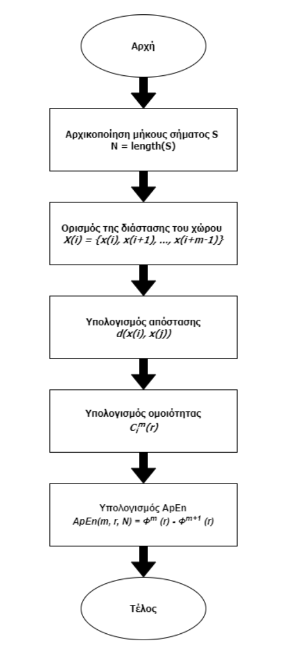
\includegraphics{ApEn.png}    
	\caption{Βήματα αλγορίθμου της \en Approximate Entropy \gr }
\end{figure}

\subsubsection{ \en Sample Entropy \gr}
Οι \en Richman \& Moorman \gr πρότειναν το 2000 τη \en Sample Entropy \gr ως έναν αλγόριθμο με δυνατότητα κάλυψης των αδυναμιών της \en Approximate Entropy. \gr Εξαρτάται και αυτή από τις ίδιες τρεις παραμέτρους και ορίζεται ως ο αρνητικός λογάριθμος της πιθανότητας: αν δύο σύνολα διάστασης $m$ έχουν απόσταση $\leq r$, τότε δύο σύνολα διάστασης $m + 1$, θα έχουν επίσης διαφορά $\leq r$. Συμβολίζεται με $SampEn(m, r, N)$ ή $SampEn(m, r, τ , N)$ αν ληφθεί υπόψιν ο χρόνος δειγματοληψίας $\tau$ . Ο αλγόριθμος αρχίζει να φιαφέρει από αυτόν της $ApEn$ από το σημείο ορισμού των $C_i ^ m (r)$ και μετά, όπου αντικαθίστανται από τα $n_m (r)$ και $n_m+1 (r)$, τις πιθανότητες ένα σημείο να είναι όμοιο με ένα άλλο στις διαστάσεις $m$ και $m+1$ αντίστοιχα:
\begin{equation}
	n_m (r) = \sum_{j=1}{N-m} \Theta (i, j, m, r), i \neq j
\end{equation}
\begin{equation}
	n_m+1 (r) = \sum_{j=1}{N-m} \Theta (i, j, m+1, r), i \neq j
\end{equation}
όπου
\begin{equation}
	\Theta (i, j, m, r) = \begin{cases}
		1, & \text{αν $||x_i - x_j||_m \leq r, j \leq i$}.\\
		0, & \text{αλλιώς}.
	\end{cases}
\end{equation}
Η \en Sample Entropy \gr δίνεται από το λόγο
\begin{equation}
	\begin{aligned}
		SampEn (m, r) = ln \frac{B^m (r)}{A^m (r)} = \lim_{N \to \infty} - \log [\frac{A^m (r)}{B^m (r)}] = \\ 
		\lim_{N \to \infty} - \log [\frac{\frac{1}{N-m} \sum_{i=1}^{N-m} A_i ^m (r)}{\frac{1}{N-m} \sum_{i=1}^{N-m} B_i ^m (r)}]
	\end{aligned}
\end{equation}
Τα $B^m (r)$ είναι η πιθανότητα δυο ακολουθίες να είναι όμοιες στη διάσταση $m$ και τα $A_m(r)$ είναι η πιθανότητα δύο ακολουθίες να είναι όμοιες στη διάσταση $m + 1$ και αποτελούν το μέσο όρο των αθροισμάτων των όρων $B_i ^m (r)$ και $Α_i ^m (r)$ που μετρούν την ομοιότητα των όρων στις αντίστοιχες διαστάσεις.
\begin{equation}
	B_i ^m (r) = \frac{1}{N - m + 1} n_m , i = 1, ..., N - m
\end{equation}
\begin{equation}
	A_i ^m (r) = \frac{1}{N - m + 1} n_m+1 , i = 1, ..., N - m
\end{equation}
Οι $SampEn$ και $ApEn$ έχουν τρεις διαφορές. Πρώτον, η $SampEn$ θεωρείται ανεξάρτητη του
μήκους $Ν$, δε συγκρίνει δηλαδή το διάνυσμα υπό μελέτη με τον εαυτό του. Δεύτερον, το άθροισμα των διανυσμάτων της βρίσκεται εντός του λογαρίθμου, ενώ στην $ApEn$ βρίσκεται εκτός. Η ανισότητα του $Jensen$ λέει ότι $\log (\sum) > \sum \log$ και αυτός ο όρος είναι μεγαλύτερος στη $SampEn$. Τέλος, η $ApEn$ περιέχει τον παράγοντα $\frac{1}{N-m}$, που την κάνει εξαρτώμενη από το $Ν$, σε αντίθεση με την $SampEn$. Ανεξαρτήτως από τις διαφορές τους, τα αποτελέσματα και των δύο εξαρτώνται εξίσου από τις άλλες δύο παραμέτρους $m, r$ και την τιμή που αυτές θα λάβουν. Επιπλέον, στη $SampEn$ όπως και στη $ApEn$, υψηλές τιμές δηλώνουν ανεξάρτητα δεδομένα, χωρίς επαναλήψεις και χαμηλές τιμές δείχνουν επανάληψη και μεγαλύτερη προβλεψιμότητα. Μια γενική σύγκριση των
τύπων παρουσιάζεται εδώ:
\begin{equation}
	\begin{aligned}
		SampEn (m, r, N) = \\
		- \log \frac{\sum_{i=1}^{N-m} \sum_{j=1 , j\neq i}^{N-m} \text{αριθμός φορών που ισχύει } d[| x_m+1 (j) - x_m+1 (i) |] < r}{\sum_{i=1}^{N-m} \sum_{j=1 , j\neq i}^{N-m} \text{αριθμός φορών που ισχύει } d[| x_m (j) - x_m (i) |] < r}
	\end{aligned}
\end{equation}
\par
\begin{equation}
	\begin{aligned}
		ApEn (m, r, N) \simeq - \frac{1}{N-m} \\
		\sum_{i=1}^{N-m} \log \frac{\sum_{j=1}^{N-m} [\text{αριθμός φορών που ισχύει } d[| x_m+1 (j) - x_m+1 (i) |] < r]}{\sum_{j=1}^{N-m} [\text{αριθμός φορών που ισχύει } d[| x_m (j) - x_m (i) |] < r]}
	\end{aligned}
\end{equation}
\par
Ακολουθεί ένα παράδειγμα χρήσης της $SampEn$. Έστω η χρονοσειρά $Ξ(Ν) = {0.1, 0.1, 0.2, 0.5,
	0.22}$ και έστω $m = 2, r = 0.2$ και $ N = 5$. Το μέγεθος του $A^m(r)$ είναι $Ν$ και του $B^m(r) Ν-1$. Άρα οι ακολουθίες για τα $A^m(r)$ και $B^m(r)$, αντίστοιχα, είναι $ \{0.1, 0.1, 0.2, 0.5, 0.22\}$ και $\{0.1, 0.1, 0.2, 0.5\}$. Για $m = 2$ οι πιθανές ακολουθίες είναι $\{(0.1, 0.1, 0.2), (0.1, 0.2, 0.5)\}$, \\
$\{(0.1, 0.1, 0.2), (0.2, 0.5, 0.22)\}, \{(0.1, 0.2, 0.5), (0.2, 0.5, 0.22)\}$. Σύμφωνα με την εξίσωση: 
\begin{equation}
	SampEn (m, r, N) = - \ln{\frac{A}{B}}
\end{equation}
\begin{equation}
	A = \frac{[(n - m - 1)(n - m)]}{2} A^m (r)
\end{equation}
\begin{equation}
	B = \frac{[(n - m - 1)(n - m)]}{2} B^m (r)
\end{equation}
H $SampEn$ υπολογίζεται ως: 
\begin{equation}
	SampEn (0, 0.2, 5) = p(0) = - \ln{\frac{A[0]}{(N * N - 1)/2}} = - \ln{610} = 0.5108
\end{equation}
\begin{equation}
	SampEn (1, 0.2, 5) = p(1) = - \ln{\frac{A[1]}{B[0]}} = - \ln{\frac{1}{3}} = 1.0986
\end{equation}
\begin{equation}
	SampEn (2, 0.2, 5) = p(2) = - \ln{\frac{A[2]}{B[1]}} = - \ln{0} = \infty
\end{equation}
\par
H $SampEn$ χρησιμοποιεί ολοκληρώματα συσχέτισης που ορίζονται στη θεωρία του χάους ως η μέση πιθανότητα δύο καταστάσεων σε δύο διαφορετικές στιγμές να βρίσκονται κοντά η μία στην άλλη.
\begin{equation}
	C(\varepsilon) = \lim_{N \to \infty} \frac{1}{N^2} \sum_{i, j = 1, i \neq j}^{N} \Theta (\varepsilon - || \overrightarrow x (i) - \overrightarrow x (j)||), \overrightarrow x (i)   \epsilon  \Re^m
\end{equation}
$N$ είναι ο αριθμός των υποτιθέμενων καταστάσεων, $\epsilon$ το κατώφλι της απόστασης.
\par
Ακόμη και αν διαφέρουν σε δομή και μαθηματικό υπόβαθρο, το συμπέρασμα είναι πως τόσο
$SampEn$ όσο και η $ApEn$ αποτελούν μεθόδους εκτίμησης πολυπλοκότητας χρονοσειρών και επηρεάζονται εξίσου από την τιμή των παραμέτρων $m, r$, η λάθος επιλογή των οποίων οδηγεί σε ανακριβή αποτελέσματα και για τις δύο. Με την πάροδο του χρόνου άλλες βελτιωμένες μορφές της $SampEn$ έχουν προταθεί [61]-[62], [67]-[69].
\subsubsection{\en Bubble Entropy \gr}
Η \en Bubble Entropy \gr αποτελεί μια νέα μετρική σχετικά με τη μέτρηση της εντροπίας σχετικής με το \en HRV. \gr Η βασική της διαφορά σε σχέση με τις προαναφερθείσες \en ApEn \gr και \en SampEn \gr είναι η μειωμένη της εξάρτηση από τις παραμέτρους $m, r$. Πιο συγκεκριμένα, η εξάρτησή της από την παράμετρο $r$ είναι μηδενική και όσον αφορά τη $m$, η σημαντικότητά της έχει μειωθεί.
\par 
Η απεξάρτηση από την $r$ έγινε εφικτή μέσω της συμβολικής ανάλυσης (Σχήμα 3.5). Στην \en Bubble Entropy \gr το εύρος τιμών της χρονοσειράς χωρίζεται σε διαστήματα που ονομάζονται από κάποια σύμβολα, όπως παραδείγματος χάριν τα γράμματα της αλφαβήτου. Τα στοιχεία λαμβάνουν το όνομά τους από το διάστημα στο οποίο ανήκουν και η αντιστοίχηση αυτή δίνει την τιμή της εντροπίας. Το μέγεθος των λέξεων καθορίζεται από την παράμετρο $m$, που αντιστοιχεί στη διάσταση του χώρου. Η σύνδεση των "ονομάτων" είναι εφικτή μέσω της κατάστασης: πανομοιότυπα/ίδια ή διαφορετικά. 
\par
Το μέγεθος των διαστημάτων κατέληξε να αντικαταστήσει την παράμετρο $r$. Για να αποβληθεί η εξάρτηση, πρέπει ο διαχωρισμός των διαστημάτων να μην είναι καθορισμένος. Το πρόβλημα αυτό λύνεται με την ενσωμάτωση της χρονοσειράς στο $m$-διάστατο χώρο. Μετά από αυτό το βήμα, κάθε διάνυσμα αντιστοιχίζεται σε ένα σημείο στο χώρο ($m$-διάστατο) και τα διαστήματα διαχωρισμού καθορίζονται με βάση τις τιμές του διανύσματος. Κάθε τιμή του διανύσματος λαμβάνει το όνομα του διαστήματος στο οποίο ανήκει, μετατρέποντας το διάνυσμα σε μια λέξη από σύμβολα μήκους $m$.
\begin{figure}[h!]
	\centering
	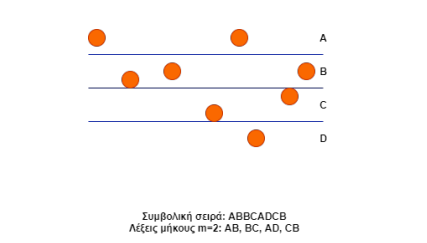
\includegraphics[scale = 0.7]{Bubble.png}    
	\caption{\gr Συμβολική ανάλυση με λέξεις μήκους $m = 2$}
\end{figure}

Όπως μπορεί να παρατηρηθεί, γίνεται κατανοητή η μοναδικότητα της κάθε λέξης, και η μοναδική της εμφάνιση. Επιπλέον, τα σύμβολα που χρησιμοποιούνται για την παραγωγή των λέξεων ανήκουν στο διάστημα [1, $m$] και το κάθε σύμβολο αντιστοιχεί στη θέση που θα είχε το εκάστοτε στοιχείο του διανύσματος αν είχε ταξινομηθεί. H διαδικασία αυτή ορίζει την πολυπλοκότητα στην οποία βασίστηκε ο αλγόριθμος της εν λόγω μετρικής. Ο αλγόριθμος που χρησιμοποιήθηκε είναι ο \en Bubble sort, \gr από τον οποίο προέρχεται και το όνομα της \en Bubble Entropy. \gr Κατά τον υπολογισμό της καταγράφεται ο αριθμός των απαιτούμενων αλλαγών για την ταξινόμηση του κάθε διανύσματος ξεχωριστά. Τα βήματα αυτά εκφράζουν μια πολυπλοκότητα, τα οποία καθιστούν την \en Bubble Entropy \gr μέθοδο εκτίμησης εντροπίας. 
\par
Τα βήματα που ακολουθεί ο αλγόριθμος είναι τα εξής  (Σχήμα 3.6):
\begin{itemize}
	\item Ενσωμάτωση του σήματος στο χώρο διάστασης $m$.
	\item Μέτρηση πλήθους αλλαγών (\en swaps \gr) για την ταξινόμηση του κάθε διανύσματος.
	\item Δημιουργία νέας ακολουθίας με το πλήθος των αλλαγών. 
	\item Εκτίμηση εντροπίας με βάση την εντροπία του \en Renyi \gr για το κάθε διάνυσμα.
	\item Επανάληψη των βημάτων για τη διάσταση $m + 1$. 
\end{itemize}
Μετά τον υπολογισμό των βημάτων, η \en Bubble Entropy \gr λαμβάνει την τιμή της από τη διαφορά εντροπίας ανάμεσα στις διαστάσεις $m$ και $m + 1$.
Όπως και οι δύο προηγούμενες μετρικές, η \en Bubble Entropy \gr υπολογίζει τη διαφορά εντροπίας ανάμεσα στους δύο πολυδιάστατους χώρους που διαφέρουν κατά ένα. Η χρήση της εντροπίας \en Rényi \gr τονίζει τις απότομες αλλαγές που περιέχονται στα σήματα, λόγω της δεύτερης τάξης που περιέχει. 
\par
Τέλος, έχει αποδειχθεί το πλεονέκτημα της ανοχής της σε έντονες κορυφές (\en "spikes"\gr) που περιέχονται σε καρδιακά σήματα κατά την καταγραφή από ΗΚΓ, το οποίο είναι μεγαλύτερο σε σύγκριση με τη \en Sample Entropy, \gr μετά την προσθήκη τεχνητού θορύβου. Στη συνέχεια, καθορίστηκε η τιμή των παραμέτρων και υπολογίστηκε η τιμή λάθους ανάμεσσα στις δύο μεθόδους. Σε κάθε περίπτωση, το λάθος της \en Bubble Entropy \gr ήταν μικρότερο από αυτό της \en Sample Entropy. \gr Οι δυνατότητες της \en Bubble Entropy \gr έχουν αποδειχθεί και σε μια προσπάθεια σύγκρισής της με την \en Permutation Entropy. \gr Οι ερευνητές συνέκριναν τις ομοιότητες και τις διαφορές των δύο μετρικών. Παραδείγματος χάριν, οι ακολουθίες ${2, 4, 6}, {6, 2, 4}$ είναι διαφορετικές για την \en Permutation Entropy \gr αλλά ίδιες για την \en Bubble Entropy \gr μιας και απαιτείται ο ίδιος αριθμός εναλλαγών για την ταξινόμησή τους.

\begin{figure}[!ht]
	\centering
	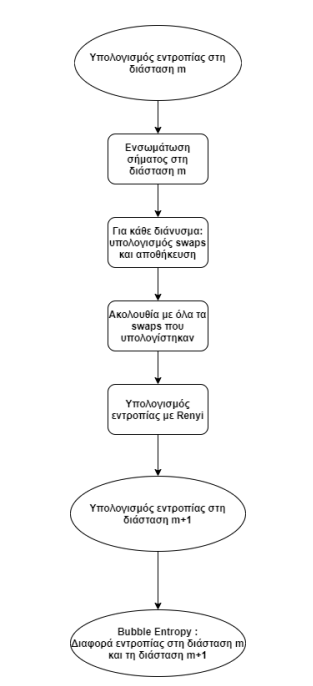
\includegraphics[scale = 0.5]{Bubble2.png}    
	\caption{Τα βήματα του αλγορίθμου της \en Bubble Entropy\gr }
\end{figure}

Πραγματοποιήθηκαν δύο σειρές πειραμάτων· στην πρώτη σειρά ερευνήθηκαν οι μεταξύ τους διαφορές και στη δεύτερη υπολογίστηκε η μεταξύ τους συνέργεια, συνδυάζοντας και τις δύο σε μια σύνθετη μέθοδο ομαδοποίησης, με εύρος διαφορετικών δεδομένων που προήλθαν τόσο από ηλεκτροκαρδιογράφημα όσο και από ηλεκτροεγκεφαλογράφημα, για την εξαγωγή πιο ολοκληρωμένων αποτελεσμάτων. 
\par
Η πρώτη σειρά πειραμάτων έδειξε πως οι δύο μέθοδοι δρούσαν με συμπληρωματικό τρόπο. Το ίδιο αποδείχθηκε και για τα δυνατά σημεία και των δύο μεθόδων. Όσον αφορά στην ακρίβειά τους στα διαφορετικά σήματα, η \en Permutation Entropy \gr έδειξε μια υπεροχή σε αυτά με περισσότερη ομαλότητα, ενώ η \en Bubble Entropy \gr στα σήματα με πιο απότομες διακυμάνσεις. 
\par
Στη δεύτερη σειρά πειραμάτων, τα αποτελέσματα ήταν ανάλογα με
το είδος των εξεταζόμενων σημάτων. Η νέα μέθοδος μπορούσε σε μερικές περιπτώσεις να ομαδοποιήσει τα σήματα πιο αποτελεσματικά από ό,τι η κάθε μέθοδος ξεχωριστά, αν και αυτό δεν υφίστατο σε όλες τις περιπτώσεις. Θεωρήθηκε, λοιπόν, πως αυτή η περίπτωση χρίζει αναλυτικότερης και βαθύτερης μελέτης. 
\par 
Ως τελευταίο παράδειγμα αναφοράς της ικανότητας της \en Bubble Entropy \gr μπορεί να ληφθεί η προσωπική μου προπτυχιακή εργασία επάνω στη μελέτη της ανθεκτικότητάς της σε τεχνητό θόρυβο. Σε αυτή την εργασία δημιουργήθηκαν τεχνητοί έκτοποι παλμοί σε πραγματικά δεδομένα τα οποία λήφθηκαν από τη βάση δεδομένων του \en PhysioNet \gr και μελετήθηκε η ανεκτικότητα της \en Bubble Entropy \gr σε σύγκριση με τις \en Approximate Entropy \gr και \en Sample Entropy \gr στο θόρυβο που προκαλούσαν αυτα τα σήματα. Σχεδόν σε όλες τις σειρές πειραμάτων που δημιουργήθηκαν, η \en Bubble Entropy \gr έδειχνε πολυ ταχύτερη σύγκλιση και σταθερότητα σχετικά με τις άλλες δύο μεθόδους εκτίμησης εντροπίας, γεγονός που ενισχύει τη χρησιμότητά της και τις δυνατότητες που διαθέτει στην εκτίμηση της εντροπίας σε καρδιακά σήματα [69]-[71], [74]. 

\subsubsection{ \en Multiscale Entropy \gr }
Aποτελεί αλγόριθμο εκτίμησης πολυπλοκότητας πεπερασμένων σειρών. Χρησιμοποιείται σε συνδυασμό με τη \en Sample Entropy, \gr η οποία βασίζεται στην εκτίμηση της προβλεψιμότητας της χρονοσειράς, όπως έχει προαναφερθεί. Το κενό αυτό καλύπτει η \en Mutiscale Entropy. \gr Στα δύο στάδια του αλγορίθμου, εφαρμόζεται ένας αδρός διαμοιρασμός στη χρονοσειρά, συχνά παραπάνω από μια φορά (σε κάθε νέα χρονοσειρά, τα σημεία της αποτελούνται από συνδυασμό 2 ή περισσότερων σημείων της προηγούμενης χρονοσειράς).
\par
\begin{figure}[!ht]
	\centering
	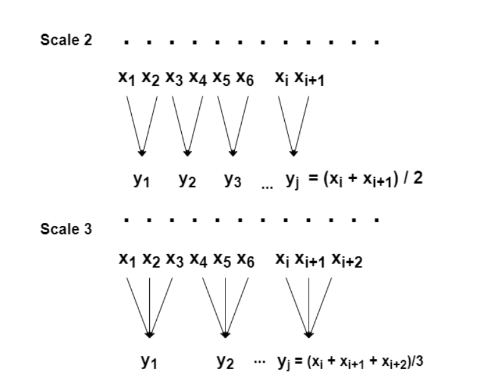
\includegraphics{Multiscale.png}    \caption{Βήματα αλγορίθμου της \en Multiscale Entropy \gr }
\end{figure}
\par
Στο δεύτερο στάδιο, εφαρμόζεται η \en Sample Entropy \gr σε κάθε μία πό τις χρονοσειρές. Η \en Sample Entropy \gr αναζητά επαναλαμβανόμενα μοτίβα σε μια χρονοσειρά και υπολογίζει την προβλεψιμότητα της χρονοσειράς. Ένα πρόβλημα που προκύπτει κατά την εφαρμογή της \en Multiscale Entropy \gr είναι το μέγεθος των δεδομένων. Για να ληφθούν σωστά τα αποτελέσματα χρειάζεται πραγματοποίηση ελέγχου στις μεγαλύτερες χρονικές κλίμακες. Στο αντίστοιχο διάγραμμα εμφανίζονται περιληπτικά τα βήματα του αλγόριθμου της \en Multiscale Entropy (Σχήμα 3.7). [72]-[73] \gr
